\chapter{Streaming}
\label{chapter:streaming}

When rendering BTF in a web-browser, all the data has to be transferred before the rendering.
Even the compressed BTF data can be tens of megabytes in size take considerable amount of time for full transmission.
We propose to stream the BTF data to reduce the delay before rendering can start,
by implementing a streaming technique.
 The user will be able to see a low quality preview of the original BTF just in a few seconds. 
In our case, principal components are streamed one by one using WebSockets technology \cite{WebSockets}.
Each principal component cover full angular domain, so the BTF can be rendered for any camera and light direction at certain point of the streaming process.
The rendering quality is enhanced whenever a new component arrives.
 Also, we provide the information about the overall progress of the stream to give an instant feedback to the user.
 
\subsection{WebSockets}
\label{chapter:sockets}

 WebSockets technology is an efficient and an elegant way of communicating between the server and the client.
 WebSockets is a brand new technology and already supports natively by web-browsers, including mobile devices.
 
This technology has several advantages over HTTP Polling, Long Polling, Streaming approaches. Main properties of WebSockets are  \cite[Ch.\ 1]{WebSockets}:

\begin{itemize}
  \item \textbf{Single connection}
   using WebSockets allow the client to reuse the same connection with the server. Whenever the new data becomes available the server sends a message to the client.
Unlike Polling method, which makes requests at regular intervals to the server to check whether the new information is available.
 This single connection reduces the latency.
 HTTP Streaming method also keeps single connection as WebSockets, but the drawback of HTTP Streaming is that it never signals if the HTTP response is finished.
 This makes harder for the client to understand if the data transmission is finished. Also, the client's firewall may buffer the HTTP response, which can result in increased latency.
  WebSockets save bandwidth, CPU power, and latency compared to HTTP Streaming, Polling methods.
  \item \textbf{Native binary data} transmission support. For instance, using binary format can decrease the size of the data compared to Base64 representation.
  This may reduce the load on the network by transferring less data.
    \item \textbf{Messaging} support after the connection is established. When the connection is open, the server and the client can send messages to each other without additional overhead.
	So, for example, the client can message the server that he needs a new principal component of the BTF.
 \item \textbf{The dedicated server} for WebSockets may perform better than traditional HTTP server. 
 Traditional servers designed for request/response cycle and may not handle properly many connections at the same \cite{tutorialWebSocket}.
 On the other hand, WebSockets server can be developed in a efficient way to handle many clients at the same time and providing so called non-blocking IO.
 For instance, NodeJs server side implementation  \cite{nodejs}.
 \end{itemize}

    
In summary, WebSockets is quite new and innovative technology. 
 It provides a big step forward in developing real-time web-applications.
 WebSockets can yield reduction in HTTP header traffic and reduction in latency compared to HTTP Polling, Streaming methods \cite[Ch.\ 1]{WebSockets}.
Overall, it is a promising technology for web-applications.


\subsection{Transmission}
\label{chapter:transmission}

\begin{figure}[h]
 \centering
 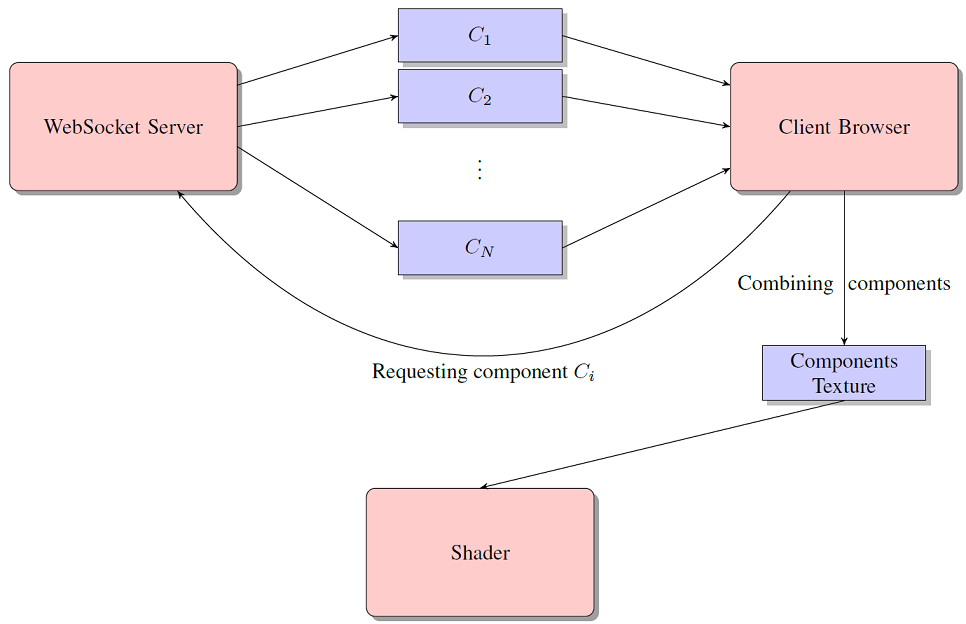
\includegraphics[width=1.0\textwidth]{figures/streaming}
 \caption[Streaming process illustration ] {
 	{\bf Streaming process illustration}
	}
 \label{fig:streaming}
\end{figure}

As it was mentioned above, for WebSockets technology the dedicated streaming server is required.
It means that the implementation code is required for the server part, in order it can properly communicate with clients and send them the requested data.
 For example, if the client requests certain BTF data, then the server should send principal components one by one. 
 The client can message the server if the component is already transferred and the server can send the next one. 
 Also, the streaming server can store all additional parameters needed for the BTF decompression.


In Section \ref{section:algorithm_step} matrices $U$, $\Sigma$ and $V$ store all the data  needed to render the BTF.
Matrices $\Sigma$ and $V$ are small in size and they are sent in the first place. On the contrary, most of the information is stored in the matrix $U$, which stores principal components.
On the client side before streaming, matrix $U$ is initialized with blank values, for example zeros. 
After the Socket connection is established, the client messages the server to send one component at a time. 
 Each component on the WebSockets server is stored as a PNG image, which provides further compression for the BTF.
When a new component fully transferred to the client, it saved to the matrix $U$ and the rendering of the BTF is refreshed.
With each component the quality of the resulting image is progressively enhanced.
Now, with streaming the client is able to see rendered image just in a few seconds.
All matrices on the client are sent to the shader as PNG images.

 The Figure \ref{fig:streaming} illustrates the described streaming process. 
 Components Texture in the Figure \ref{fig:streaming} is the matrix $U$, which saves the transferred principal components.









